\chapter{The scattering formula in the plane--sphere geometry}
\label{chapter_scattering_ps}

\begin{wrapfigure}{r}{0.382\textwidth}
\begin{center}
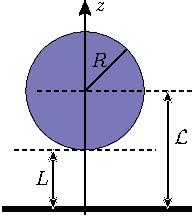
\includegraphics[scale=1.5]{images/geometry.pdf}
\end{center}
\caption{Sphere of radius $R$ and plate separated by a distance $L$ with
center-to-plate distance $\L \equiv L+R$.}
\label{fig:4_geometry}
\end{wrapfigure}

In this chapter, we apply the scattering formula to the plane--sphere geometry.
The plate is located at $z=0$ and assumed to be infinite in the $xy$--plane.
The center of the sphere is located above the plate at $z= L+R \equiv
\mathcal{L}$, where $R$ is the radius of the sphere and $L$ is the distance
between the plate and the sphere. The geometry is shown in
Fig. \ref{fig:4_geometry}. Moreover, we assume plate and sphere to be thick
enough to be considered as bulk.

We derive the matrix elements of the scattering operator in the multipole basis
and perform a Wick rotation. The free energy $\F$ depends on temperature, the
reflection properties of plate and sphere, the sphere's radius $R$ and the
separation $L$. We study the contribution to the free energy for the Matsubara
frequency $\xi=0$ in more detail, because the numerical evaluation causes
problems. Given the free energy $\F(L,T)$, we can derive the force $F$ and the
entropy $S$ by
\begin{equation}
F = - \frac{\partial \F}{\partial L}, \\ S = - \frac{\partial \F}{\partial T}.
\end{equation}

We follow the reasoning of \textsc{Durand} et al. \cite{Durand,
ThermalCasimirEffect} to derive the matrix elements of the round-trip operator.
However, we want to be more rigorous and explicit in our line of argumentation.
Although equivalent, our matrix elements will differ from those of
\textsc{Durand} et al. and avoid Wigner (small) d-matrix elements. Moreover,
the matrix elements have symmetries that can be exploited to decrease
computational effort.

The Casimir effect in the plane--sphere geometry contains five length scales:
the geometrical scales $L$ and $R$, the thermal wavelength $\lambda_T =
\hbar\c/\kb T$, the plasma wavelength $\lambda_P=2\pi\c/\omega_P$, and the
wavelength $\lambda_\gamma = 2\pi\c/\gamma$ associated with the finite
conductivity of the metals. We scale the quantities involved and show that only
four length scales are independent. In particular, the free energy for perfect
mirrors depends only on the temperature and the ratio of $L$ and $R$:
$\mathcal{F} = \mathcal{F}(T,L/R)$. In the last section, we give a conclusion
and present the results of this chapter in condensed form.


\section{Round-trip operator $\mathcal{M}$}

In the plane--sphere geometry, the round-trip operator consists of the
translation operator from sphere to plane
$\mathcal{T}_{\text{P}\leftarrow\text{S}}$, the reflection operator at the
plane $\mathcal{R}_\text{P}$, the translation operator from plane to sphere
$\mathcal{T}_{\text{S}\leftarrow\text{P}}$, and the reflection operator at the
sphere $\mathcal{R}_\text{S}$:
\begin{equation}
\mathcal{M}(\omega) = \mathcal{R}_\text{S}(\omega) \mathcal{T}_{\text{S}\leftarrow\text{P}}(\omega) \mathcal{R}_\text{P}(\omega) \mathcal{T}_{\text{P}\leftarrow\text{S}}(\omega)
\end{equation}
The round-trip operator represents a round trip within the cavity.
Except for
the temperature, $\mathcal{M}$ contains the whole information about
the physical system: The separation $L$ of sphere and
plate affects the translation operators
$\mathcal{T}_{\text{S}\leftarrow\text{P}}$ and
$\mathcal{T}_{\text{P}\leftarrow\text{S}}$, the radius $R$ of the sphere and the
reflection properties of the sphere enter the reflection operator
$\mathcal{R}_\text{S}$, and the reflection properties of the plane enter
$\mathcal{R}_\text{P}$.

Before we express the round-trip operator in the multipole basis, let us first
take a look at the symmetries of the plane--sphere configuration: The
configuration is time invariant, so the frequency $\omega$ is preserved during
a round trip. Moreover, the geometry is invariant under rotations around the
$z$-axis and the round-trip operator $\mathcal{M}$ commutes with the angular
momentum operator $\hat J_z$. Therefore, the round-trip operator $\mathcal{M}$
is block-diagonal with respect to $m$ and each block $\mathcal{M}^{(m)}$ yields
an independent contribution to the free energy
\begin{equation}
\F = \kb T {\sum_{n=0}^\infty}^\prime \sum_{m=-\infty}^\infty \log \det \left[\Id - \mathcal{M}^{(m)}(\omega) \right].
\end{equation}
The conservation of $m$ is discussed in more detail in appendix \ref{appendix_conserved_m}.


\section{Round-trip operator in multipole basis}

We want to express the matrix elements of $\mathcal{M}$ in the multipole basis.
The multipole basis is well adapted to the rotational symmetry around the
$z$-axis and $\mathcal{M}$ is block diagonal with respect to $m$. Although
infinite, the rows and columns of the round-trip matrix are countable. The
round-trip operator in the multipole basis is given by
\begin{equation}
\label{eq:scattering_0}
\mathcal{M}^{(m)}_{(\ell_1,P_1;\ell_2,P_2)}(\omega) = \braket{\ell_1,m,P_1 \, | \, \mathcal{R}_\text{S} \mathcal{T}_{\text{S}\leftarrow\text{P}} \mathcal{R}_\text{P} \mathcal{T}_{\text{P}\leftarrow\text{S}} \, | \, \ell_2,m,P_2}.
\end{equation}

When acting on plane waves, the
translation operators yield phase factors
\begin{equation}
\mathcal{T}_{\text{P}\leftarrow\text{S}} \ket{\, \vec k, p, \phi} = \e^{-\imag \phi k_z \mathcal{L}} \ket{\, \vec k, p, \phi}, \\
\mathcal{T}_{\text{S}\leftarrow\text{P}} \ket{\, \vec k, p, \phi} = \e^{+\imag \phi k_z \mathcal{L}} \ket{\, \vec k, p, \phi},
\end{equation}
that depend on the direction of propagation.
The reflection operator at the plane yields
\begin{equation}
\mathcal{R}_\text{P} \ket{\, \vec k, p, +} = 0, \\
\mathcal{R}_\text{P} \ket{\, \vec k, p, -} = r_p(\omega, \vec k) \ket{\, \vec k, p, +},
\end{equation}
where $r_p$ is a Fresnel coefficient.

Let us insert the identity operator in the plane wave basis in
\eqref{eq:scattering_0} and evaluate the propagation from sphere to
plate:
\begin{equation}
\mathcal{M}^{(m)}_{(\ell_1,P_1;\ell_2,P_2)}(\omega) = %\sum_{p,\phi} \braket{\ell_1,m,P_1 \, | \, \mathcal{R}_\text{S} \mathcal{T}_{\text{S}\leftarrow\text{P}} \mathcal{R}_\text{P} \mathcal{T}_{\text{P}\leftarrow\text{S}} \, | \, \vec k, p, \phi}\braket{\vec k, p, \phi \, | \, \ell_2,m,P_2} \\
\sum_{p,\phi} \int \mathrm{d}^2 \vec k \, \e^{-\phi\imag k_z \mathcal{L}}\braket{\ell_1,m,P_1 \, | \, \mathcal{R}_\text{S} \mathcal{T}_{\text{S}\leftarrow\text{P}} \mathcal{R}_\text{P} \, | \, \vec k, p, \phi}\braket{\vec k, p, \phi \, | \, \ell_2,m,P_2} 
\end{equation}
The reflection operator $\mathcal{R}_p$ yields only a nonvanishing term
for waves travelling in downward direction. Therefore, the sum over $\phi$
has only one contribution for $\phi=-1$ and the reflection operator
introduces the Fresnel coefficient $r_p$. The evaluation of the
translation operator yields another phase factor and we find
\begin{equation}
\mathcal{M}_{(\ell_1,P_1;\ell_2,P_2)}^{(m)}(\omega) = \sum_{p} \int \mathrm{d}^2 \vec k \, r_p(\omega,\vec k) \, \e^{2 \imag k_z \mathcal{L}}\braket{\ell_1,m,P_1 \, | \, \mathcal{R}_\text{S} \, | \, \vec k, p, +}\braket{\vec k, p, - \, | \, \ell_2,m,P_2}.
\end{equation}
By inserting the identity operator in multipole basis, we get
\begin{align}
\nonumber
\braket{\ell,m,P \, | \, \mathcal{R}_S \, | \, \vec{k},+,p} &= \sum_{\ell^\prime=1}^\infty \sum_{m^\prime=-\ell^\prime}^{\ell^\prime} \sum_{P^\prime=\PE,\PM} \braket{\ell,m,P \, | \, \mathcal{R}_S \, | \, \ell^\prime,m^\prime,P^\prime} \braket{\ell^\prime,m^\prime,P^\prime \, | \, \vec{k},+,p} \\
&= \braket{\ell,m,P \, | \, \mathcal{R}_\text{S} \, | \, \ell,m,P} \braket{\ell,m,P \, | \, \vec{k},+,p}.
\end{align}
The operator $\mathcal{R}_\text{S}$ is diagonal in the multipole basis with
matrix elements proportional to the Mie coefficients $a_\ell$ and $b_\ell$. The
matrix elements of $\mathcal{R}_\text{S}$ are given by
\begin{equation}
\braket{\ell,m,E \, | \, \mathcal{R}_\text{S} \, | \, \ell,m,E} = -2 a_\ell(\omega), \\
\braket{\ell,m,M \, | \, \mathcal{R}_\text{S} \, | \, \ell,m,M} = -2 b_\ell(\omega),
\end{equation}
where we have used the definition of \textsc{Bohren} and \textsc{Huffman} 
for the Mie coefficients $a_\ell$, $b_\ell$ \cite{bohrenhuffman}.
The reader finds a discussion of the origin of the factor $-2$ in appendix \ref{appendix_factor2}.
We also want to point out that the Mie coefficients only depend on $\ell$ and the frequency
$\omega$, but not on $m$ or $\vec k$.

In conclusion, we find for the matrix elements of the round-trip operator
\begin{align}
\nonumber
\mathcal{M}^{(m)}_{(\ell_1,P_1;\ell_2,P_2)}(\omega) = \sum_{p={\TE,\TM}} &\int \mathrm{d}^2 \vec k \, r_p(\omega,\vec k) \, \e^{2 \imag k_z \mathcal{L}} \braket{\ell_1,m,P_1 \, | \, \mathcal{R}_\text{S} \, | \, \ell_1,m,P_1}\\
\label{eq:scattering_roundtrip}
&\times \braket{\ell_1,m,P_1 \, | \, \vec k, p, +} \braket{\vec k, p, - \, | \, \ell_2,m,P_2}
\end{align}
and organize the round-trip matrix as a block matrix:
\begin{equation}
\mathcal{M}^{(m)}(\omega) = \left(\begin{array}{cc}
\mathcal{M}^{(m)}(E,E) & \mathcal{M}^{(m)}(E,M) \\
\mathcal{M}^{(m)}(M,E) & \mathcal{M}^{(m)}(M,M)
\end{array}
\right)
\end{equation}


\begin{figure}
\begin{center}
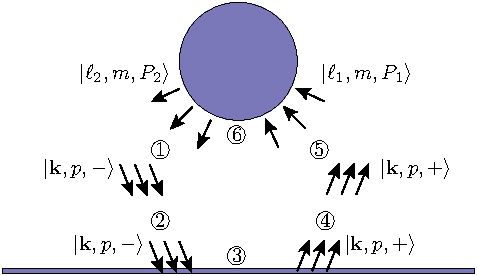
\includegraphics[scale=1.8]{images/roundtrip.pdf}
\end{center}
\caption{
Visualization of the components of the matrix elements of $\mathcal{M}$ in \eqref{eq:scattering_roundtrip}. Plane waves are used for propagation
and reflection at the plate, multipole waves are used for the reflection at the sphere. (cf. \cite{Durand})}
\label{fig:scattering_roundtrip}
\end{figure}

Eq. \eqref{eq:scattering_roundtrip} has a simple interpretation when read
from right to left (cf. Fig. \ref{fig:scattering_roundtrip}):

\begin{enumerate}[label=\protect\circled{\arabic*}]
\item $\braket{\vec k, p, - \, | \, \ell_2,m,P_2}$:
The multipole wave $\Ket{\ell_2,m,P_2}$ is decomposed into plane waves.

\item $\e^{\imag k_z \mathcal{L}}$:
The plane waves $\ket{\vec k, -, p}$ propagate the distance $\mathcal{L}$
towards the plate. The propagation yields a phase factor $\e^{\imag k_z
\mathcal{L}}$.

\item $r_p(\omega,\vec k)$:
The plane waves $\Ket{\vec k, p, -}$ are reflected at the plate. The reflection
preserves the wave vector $\vec k$ and the polarization~$p$, but
changes the direction of propagation. The reflection coefficient is given
by the Fresnel coefficient $r_p$.

\item $\e^{\imag k_z \mathcal{L}}$:
The plane waves $\ket{\vec k, +, p}$ propagate the distance $\mathcal{L}$
towards the sphere.

\item $\braket{\ell_1,m,P_1 \, | \, \vec k, p, +}$:
The plane waves $\ket{\vec k, +, p}$ are decomposed into multipole waves
$\ket{\ell_1,m,P_1}$.

\item $\braket{\ell_1,m,P_1 \, | \, \mathcal{R}_\text{S} \, | \, \ell_1,m,P_1}$:
The multipole waves are reflected at the sphere. The reflection preserves
polarization, total angular momentum and the $z$-component of the angular
momentum. In conclusion, the quantum numbers $\ell$, $m$ and $P_1$ are
preserved.
\end{enumerate}


\section{Matrix elements in multipole basis}

In this chapter, we derive explicit matrix elements for the scattering matrix.
We substitute the spherical harmonics in the matrix elements performing the
change of basis \eqref{eq:basis_change_1}--\eqref{eq:basis_change_4} by
associated Legendre polynomials:
\begin{align}
\Ylm{\ell m}(\theta^\pm, \varphi) &= \Nlm{\ell m} \Plm{\ell}{m}(\cos\theta^\pm) \frac{\e^{\imag m \varphi}}{\sqrt{2\pi}} = \Nlm{\ell m} \Plm{\ell}{m}\left(\pm \frac{\c k_z}{\omega}\right) \frac{\e^{\imag m \varphi}}{\sqrt{2\pi}} \\
\partial_\theta \Ylm{\ell m}(\theta^\pm, \varphi) &= \Nlm{\ell m} \Plm{\ell}{m}^\prime(\cos\theta^\pm) (-\sin\theta^\pm) \frac{\e^{\imag m \varphi}}{\sqrt{2\pi}} 
= - \frac{\c k}{\omega} \Nlm{\ell m} \Plm{\ell}{m}^\prime\left(\pm \frac{\c k_z}{\omega}\right) \frac{\e^{\imag m \varphi}}{\sqrt{2\pi}} 
\end{align}
Properties of spherical harmonics and associated Legendre polynomials, and the
definition of the normalizing constant $\Nlm{\ell m}$ can be found in the
sections \ref{appendix_sfunc_spherical_harmonics} and
\ref{appendix_sfun_assoc_legendre} of the appendix. As the geometry is
invariant under rotations around the $z$-axis, the matrix elements become
independent of $\varphi$. An integration over $\varphi$ yields $2\pi$ and the
matrix elements are given as an integral over $k$
\begin{align}
\mathcal{M}^{(m)}(E,E)_{\ell_1 \ell_2} &= \phantom{-}\Lambda^{(m)}_{\ell_1 \ell_2} a_{\ell_1}(\omega) \left[ A^{(m)}_{\ell_1 \ell_2,\TE}(\omega)+ B^{(m)}_{\ell_1 \ell_2, \TM}(\omega)\right], \\
\mathcal{M}^{(m)}(M,M)_{\ell_1 \ell_2} &= \phantom{-}\Lambda^{(m)}_{\ell_1 \ell_2} b_{\ell_1}(\omega) \left[ A^{(m)}_{\ell_1 \ell_2,\TM}(\omega)+ B^{(m)}_{\ell_1 \ell_2, \TE}(\omega)\right], \\
\mathcal{M}^{(m)}(E,M)_{\ell_1 \ell_2} &= \phantom{-}\Lambda^{(m)}_{\ell_1 \ell_2} a_{\ell_1}(\omega) \left[ C^{(m)}_{\ell_1 \ell_2,\TE}(\omega)+ D^{(m)}_{\ell_1 \ell_2, \TM}(\omega)\right], \\
\mathcal{M}^{(m)}(M,E)_{\ell_1 \ell_2} &= -\Lambda^{(m)}_{\ell_1 \ell_2} b_{\ell_1}(\omega) \left[ C^{(m)}_{\ell_1 \ell_2,\TM}(\omega)+ D^{(m)}_{\ell_1 \ell_2, \TE}(\omega)\right],
\end{align}
where we have defined the prefactor
\begin{equation}
\label{eq:4_lambda}
\Lambda_{\ell_1 \ell_2}^{(m)} \equiv \frac{-2 \, \mathrm{N}_{\ell_1 m}\,\mathrm{N}_{\ell_2 m}}{\sqrt{\ell_1 (\ell_1+1)\,\ell_2(\ell_2+1)}}
= -\sqrt{ \frac{(2\ell_1+1)\,(2\ell_2+1)\,(\ell_1-m)!\,(\ell_2-m)!}{(\ell_1+m)!\, (\ell_2+m)!\, \ell_1(\ell_1+1) \, \ell_2(\ell_2+1)} },
\end{equation}
and the integrals
\begin{align}
\label{scattering_int_A_r}
A_{\ell_1 \ell_2,p}^{(m)}(\omega) &\equiv \int_0^\infty \mathrm{d}k \, \frac{m^2}{\c k} \left|\frac{\omega}{k_z}\right| \, r_p(\omega, k) \, \e^{2\imag k_z \mathcal{L}} \, \Plm{\ell_1}{m}\left(\frac{\c k_z}{\omega}\right) \Plm{\ell_2}{m}\left(-\frac{\c k_z}{\omega}\right), \\
\label{scattering_int_B_r}
B_{\ell_1 \ell_2,p}^{(m)}(\omega) &\equiv \int_0^\infty \mathrm{d}k \, \frac{\c^3 k^3}{\omega^4} \left|\frac{\omega}{k_z}\right| \, r_p(\omega, k) \, \e^{2\imag k_z \mathcal{L}} \, \Plm{\ell_1}{m}^\prime\left(\frac{\c k_z}{\omega}\right) \Plm{\ell_2}{m}^\prime\left(-\frac{\ k_z}{\omega}\right), \\
\label{scattering_int_C_r}
C_{\ell_1 \ell_2,p}^{(m)}(\omega) &\equiv \int_0^\infty \mathrm{d}k \, \frac{\imag m \c k}{\omega^2} \left|\frac{\omega}{k_z}\right| \, r_p(\omega, k) \, \e^{2\imag k_z \mathcal{L}} \, \Plm{\ell_1}{m}\left(\frac{\c k_z}{\omega}\right) \Plm{\ell_2}{m}^\prime\left(-\frac{\c k_z}{\omega}\right), \\
\label{scattering_int_D_r}
D_{\ell_1 \ell_2,p}^{(m)}(\omega) &\equiv \int_0^\infty \mathrm{d}k \, \frac{\imag m \c k}{\omega^2} \left|\frac{\omega}{k_z}\right| \, r_p(\omega, k) \, \e^{2\imag k_z \mathcal{L}} \, \Plm{\ell_1}{m}^\prime\left(\frac{\c k_z}{\omega}\right) \Plm{\ell_2}{m}\left(-\frac{\c k_z}{\omega}\right).
\end{align}
We put the Mie coefficients $a_\ell$, $b_\ell$ in front of the integrals,
because they are independent of $k$. The reader is warned that the absolute
value functions are important to account for evanescent waves: We integrate
over $k$ for a fixed value of $\omega$. The absolute value of the
$z$-component of the wavevector is given by $k_z=\sqrt{\omega^2/\c^2-k^2}$ and
becomes imaginary for $k>\omega/\c$. Moreover, in the next chapter we perform a
Wick rotation and therefore $\omega$ will also become imaginary.

\section{Wick rotation}
\label{section_wick}

In an analog manner to the Wick rotation in the plane--plane geometry in section \ref{section_scattering_pp_free_energy}, we
rotate the axis of integration to imaginary frequencies. This Wick rotation
changes $\omega \to \imag \xi$ and $k_z \to \imag\kappa$ in the integrands and
the matrix elements of the round-trip matrix become
\begin{align}
\label{eq:4_EE}
\mathcal{M}^{(m)}(E,E)_{\ell_1 \ell_2} &= \phantom{-}\Lambda^{(m)}_{\ell_1 \ell_2} a_{\ell_1}(\imag\xi) \left[ A^{(m)}_{\ell_1 \ell_2,\TE}(\xi)+ B^{(m)}_{\ell_1 \ell_2, \TM}(\xi)\right], \\
\label{eq:4_MM}
\mathcal{M}^{(m)}(M,M)_{\ell_1 \ell_2} &= \phantom{-}\Lambda^{(m)}_{\ell_1 \ell_2} b_{\ell_1}(\imag\xi) \left[ A^{(m)}_{\ell_1 \ell_2,\TM}(\xi)+ B^{(m)}_{\ell_1 \ell_2, \TE}(\xi)\right], \\
\label{eq:4_EM}
\mathcal{M}^{(m)}(E,M)_{\ell_1 \ell_2} &= \phantom{-}\Lambda^{(m)}_{\ell_1 \ell_2} a_{\ell_1}(\imag\xi) \left[ C^{(m)}_{\ell_1 \ell_2,\TE}(\xi)+ D^{(m)}_{\ell_1 \ell_2, \TM}(\xi)\right], \\
\label{eq:4_ME}
\mathcal{M}^{(m)}(M,E)_{\ell_1 \ell_2} &= -\Lambda^{(m)}_{\ell_1 \ell_2} b_{\ell_1}(\imag\xi) \left[ C^{(m)}_{\ell_1 \ell_2,\TM}(\xi)+ D^{(m)}_{\ell_1 \ell_2, \TE}(\xi)\right],
\end{align}
with the integrals
\begin{align}
\label{scattering_int_A}
A_{\ell_1 \ell_2,p}^{(m)}(\xi) &= \frac{m^2 \xi}{\c} \int_0^\infty \mathrm{d}k \, \frac{1}{k \kappa} \, r_p(\imag\xi,k) \, \e^{-2\kappa\mathcal{L}} \, \Plm{\ell_1}{m}\left(\frac{\kappa\c}{\xi}\right) \Plm{\ell_2}{m}\left(-\frac{\kappa\c}{\xi}\right), \\
\label{scattering_int_B}
B_{\ell_1 \ell_2,p}^{(m)}(\xi) &= \frac{\c^3}{\xi^3} \int_0^\infty \mathrm{d}k \, \frac{k^3}{\kappa} \, r_p(\imag\xi,k) \, \e^{-2\kappa\mathcal{L}} \, \Plm{\ell_1}{m}^\prime\left(\frac{\kappa\c}{\xi}\right) \Plm{\ell_2}{m}^\prime\left(-\frac{\kappa\c}{\xi}\right), \\
\label{scattering_int_C}
C_{\ell_1 \ell_2,p}^{(m)}(\xi) &= -\frac{\imag m\c}{\xi} \int_0^\infty \mathrm{d}k \, \frac{k}{\kappa} \, r_p(\imag\xi,k) \, \e^{-2\kappa\mathcal{L}} \, \Plm{\ell_1}{m}\left(\frac{\kappa\c}{\xi}\right) \Plm{\ell_2}{m}^\prime\left(-\frac{\kappa\c}{\xi}\right), \\
\label{scattering_int_D}
D_{\ell_1 \ell_2,p}^{(m)}(\xi) &= -\frac{\imag m\c}{\xi} \int_0^\infty \mathrm{d}k \, \frac{k}{\kappa} \, r_p(\imag\xi,k) \, \e^{-2\kappa\mathcal{L}} \, \Plm{\ell_1}{m}^\prime\left(\frac{\kappa\c}{\xi}\right) \Plm{\ell_2}{m}\left(-\frac{\kappa\c}{\xi}\right).
\end{align}
The integrals are damped by an exponential function which ensures fast
convergence. The argument of the associated Legendre polynomials is given by
$\kappa\c/\xi \ge 1$. The Legendre polynomials can be generalized to arguments
greater than unity by analytic continuation. However, for odd values of $m$ the
analytic continuation is only unique up to a phase factor $\pm1$. Nonetheless,
when multiplying two associated Legendre polynomials (or their derivatives) of
the same order $m$, the phase factors cancel. Thus the values of the integrals
are independent of the choice of the phase factor. A brief discussion about the
analytic continuation can be found in appendix
\ref{appendix_sfun_assoc_legendre}.

Although the matrix elements of the round-trip operator look different than
those of \textsc{Durand} et al. \cite{Durand, ThermalCasimirEffect}, the matrix
elements are equivalent. In appendix \ref{appendix_umrechnung} we proof this
equivalence for the matrix element $\mathcal{M}_\TE^{(m)}(E,E)_{\ell_1\ell_2}$.
The proofs for the remaining matrix elements can be carried out in a similar
manner.


\section{Properties of the scattering matrix}

In this section, we show useful properties of the scattering matrix and its
matrix elements. We will show that the determinant of the scattering matrix is
real and that the matrix elements can be written in terms of real quantities.
Moreover, we investigate symmetries among the matrix elements that can be
exploited to decrease computational effort.

\subsection{Determinant of the scattering matrix}

All quantities in the integrands of
\eqref{scattering_int_A}--\eqref{scattering_int_D} are real except for the
associated Legendre polynomials. The product of two associated Legendre
polynomials or their derivatives for the same degree $m$ are either real or
pure imaginary for arguments $x \ge 1$. In appendix
\ref{appendix_sfun_assoc_legendre} we show that for $x\ge1$
\begin{equation}
\Plm{\ell_1}{m}(x) \Plm{\ell_2}{m}(x) \in \mathbb{R}, \\
\Plm{\ell_1}{m}^\prime(x) \Plm{\ell_2}{m}^\prime(x) \in \mathbb{R}, \\
\Plm{\ell_1}{m}(x) \Plm{\ell_2}{m}^\prime(x) \in \mathbb{R}.
\end{equation}
Hence, the block matrices $A^{(m)}_{\ell_1\ell_2}$ and $B^{(m)}_{\ell_1\ell_2}$ are
real, while $\mathcal{M}^{(m)}(E,M)$ and $\mathcal{M}^{(m)}(M,E)$
are pure imaginary.
With \eqref{eq:appendix_det_i} we can write the scattering matrix with real matrix elements
\begin{equation}
\det \mathcal{D}^{(m)} = \det \left(\begin{array}{cc}
\mathbbm{1}-\mathcal{M}^{(m)}(E,E) & -\Im{\left[\mathcal{M}^{(m)}(E,M)\right]} \\
\Im{\left[\mathcal{M}^{(m)}(M,E)\right]} & \mathbbm{1}-\mathcal{M}^{(m)}(M,M)
\end{array}\right).
\end{equation}
From this it follows immediately that the determinant is a real number. As the
energy is a real quantity, it follows from a physical point of view that the
determinant must be positive as well. However, we have not proven the last
point.


\subsection{Symmetries}

The prefactor $\Lambda_{\ell_1 \ell_2}^{(m)}$ is invariant when
interchanging $\ell_1$ and $\ell_2$.
Using this symmetry together with the parity of the
associated Legendre polynomials (cf. \eqref{appendix_sfun_assoclegendre_parity}), one can show that
\begin{equation}
A_{\ell_2 \ell_1,p}^{(m)} = (-1)^{\ell_1+\ell_2} A_{\ell_1 \ell_2,p}^{(m)}, \\
B_{\ell_2 \ell_1,p}^{(m)} = (-1)^{\ell_1+\ell_2} B_{\ell_1 \ell_2,p}^{(m)}, \\
D_{\ell_1 \ell_2,p}^{(m)} = (-1)^{\ell_1+\ell_2+1} \, C_{\ell_2 \ell_1,p}^{(m)}.
\end{equation}
By exploiting these relations, it is sufficient to evaluate
$N^2+N$ integrals for a block matrix $\mathcal{M}^{(m)}(P_1,P_2)$ of dimension $N$
instead of $2N^2$ integrals. If we consider perfect mirrors, the Fresnel coefficients
are given by $r_\TM=-r_\TE=1$ and integrals for different polarization $p=\TE,\TM$
differ only in sign
\begin{equation}
X_{\ell_1 \ell_2,\TE} = -X_{\ell_1 \ell_2,\TM},
\end{equation}
where $X=A,B,C,D$. Therefore, for perfect mirrors we just have to evaluate
$(N^2+N)/2$ integrals.

When changing from $m\to-m$ the prefactor $\Lambda$ can be expressed as
\begin{equation}
\label{eq:4_lamdamm}
\Lambda_{\ell_1 \ell_2}^{(-m)} = \frac{(\ell_1+m)!\,(\ell_2+m)!}{(\ell_1-m)!\,(\ell_2-m)!} \Lambda_{\ell_1 \ell_2}^{(m)},
\end{equation}
and the integrals \eqref{scattering_int_A}--\eqref{scattering_int_D} as
\begin{equation}
\label{eq:4_mm}
X_{\ell_1 \ell_2}^{(-m)} = \pm \frac{(\ell_1-m)!\,(\ell_2-m)!}{(\ell_1+m)!\,(\ell_2+m)!} X_{\ell_1 \ell_2}^{(m)},
\end{equation}
with $+$ for $X=A,B$ and $-$ for $X=C,D$. Indeed, we see that
\begin{equation}
\Lambda_{\ell_1 \ell_2}^{(-m)} X_{\ell_1 \ell_2}^{(-m)} = \pm \Lambda_{\ell_1 \ell_2}^{(m)} X_{\ell_1 \ell_2}^{(m)}.
\end{equation}
Hence, the diagonal blocks of the round-trip matrix are invariant for $m\to-m$
while the nondiagonal blocks change sign:
\begin{align}
\mathcal{M}^{(-m)}(\xi_n) = \left(\begin{array}{cc}
   \phantom{-}\mathcal{M}^{(m)}(E,E) &           -\mathcal{M}^{(m)}(E,M) \\
             -\mathcal{M}^{(m)}(M,E) & \phantom{-}\mathcal{M}^{(m)}(M,M)
\end{array}\right)
\end{align}
However, the determinant of the matrix $\mathcal{D}^{(m)}$ is invariant for
$m\to-m$ which is shown in appendix \ref{appendix_determinant_block_matrices}.
The summation over $m$ in the formula for the free energy can thus be limited
to non-negative values of $m$ by weighting every term but $m=0$ with a factor
$2$, and therefore the free energy becomes
\begin{equation}
\label{eq:4_Fk}
\mathcal{F} = 2\kb T {\sum_{n=0}^\infty}^\prime {\sum_{m=0}^\infty}^\prime \log\det \left[ \mathbbm{1} - \mathcal{M}^{(m)}(\xi_n)\right].
\end{equation}

Exploiting the properties of the scattering matrix we found in this section
will help to significantly reduce the computational time in a numerical
implementation.


\section{Scaling}

\label{scattering_ps_scaling}

In this master thesis, we are more interested in effects due to geometry and
temperature than in effects due to finite conductivity and dissipation of the
mirrors. For this reason, we will mainly consider perfect reflectors in the
next chapters. In the case of perfect reflectors, only two length scales are
independent. We change over to dimensionless units, which help to simplify
equations and to eliminate one length scale.

We introduce the scaled quantities:
\begin{equation}
\label{eq:scattering_ps_scaled}
\tilde{\mathcal{F}} = \frac{\mathcal{L}}{\hbar \c} \, \mathcal{F}, \\
\tilde{T}           = \frac{2\pi \kb \mathcal{L}}{\hbar \c} \, T, \\
\tilde{k}           = \mathcal{L} k, \sep \mathrm{d}\tilde{k} = \mathcal{L} \mathrm{d}k, \\
\tilde{\kappa}      = \mathcal{L} \kappa = \sqrt{n^2 \tilde{T}^2 + \tilde{k}^2} \\
\end{equation}
We also define dimensionless quantities for $\xi$, $\omega_\text{P}$ and $\gamma$:
\begin{equation}
\tilde{\xi}_n           = \frac{\xi_n \mathcal{L}}{\c} = n \tilde{T}, \\
\tilde{\omega}_\text{P} = \frac{\omega_\text{P} \mathcal{L}}{\c}, \\
\tilde{\gamma}          = \frac{\gamma \mathcal{L}}{\c}
\end{equation}
The Mie coefficients are evaluated at
\begin{equation}
\chi = \frac{n\tilde{T}R}{\mathcal{L}} = \frac{n\tilde{T}}{1+L/R}.
\end{equation}
Changing over to dimensionless quantities, the free energy becomes
\begin{equation}
\tilde{\mathcal{F}} = \frac{\tilde{T}}{\pi} {\sum_{n=0}^\infty}^\prime {\sum_{m=0}^\infty}^\prime \log\det \left[ \mathbbm{1} - \mathcal{M}^{(m)}(n\tilde T)\right]
\end{equation}
with the integrals
\begin{align}
\label{scattering_int_A_scaled}
A_{\ell_1 \ell_2,p}^{(m)}(n\tilde{T}) &= m^2 \, n\tilde{T} \int_0^\infty \mathrm{d}\tilde{k} \, \frac{1}{\tilde{k} \tilde{\kappa}} \, r_p(\imag\tilde{\xi},\tilde{k}) \, \e^{-2\tilde{\kappa}} \, \Plm{\ell_1}{m}\left(\frac{\tilde{\kappa}}{n\tilde{T}}\right) \Plm{\ell_2}{m}\left(-\frac{\tilde{\kappa}}{n\tilde{T}}\right), \\
\label{scattering_int_B_scaled}
B_{\ell_1 \ell_2,p}^{(m)}(n\tilde{T}) &= \frac{1}{(n\tilde{T})^3} \int_0^\infty \mathrm{d}\tilde{k} \, \frac{\tilde{k}^3}{\tilde{\kappa}} \, r_p(\imag\tilde{\xi},\tilde{k}) \, \e^{-2\tilde{\kappa}} \, \Plm{\ell_1}{m}^\prime\left(\frac{\tilde{\kappa}}{n\tilde{T}}\right) \Plm{\ell_2}{m}^\prime\left(-\frac{\tilde{\kappa}}{n\tilde{T}}\right), \\
\label{scattering_int_C_scaled}
C_{\ell_1 \ell_2,p}^{(m)}(n\tilde{T}) &= -\frac{\imag m}{n\tilde{T}} \int_0^\infty \mathrm{d}k \, \frac{\tilde{k}}{\tilde{\kappa}} \, r_p(\imag\tilde{\xi},\tilde{k}) \, \e^{-2\tilde{\kappa}} \, \Plm{\ell_1}{m}\left(\frac{\tilde{\kappa}}{n\tilde{T}}\right) \Plm{\ell_2}{m}^\prime\left(-\frac{\tilde{\kappa}}{n\tilde{T}}\right), \\
\label{scattering_int_D_scaled}
D_{\ell_1 \ell_2,p}^{(m)}(n\tilde{T}) &= -\frac{\imag m}{n\tilde{T}} \int_0^\infty \mathrm{d}k \, \frac{\tilde{k}}{\tilde{\kappa}} \, r_p(\imag\tilde{\xi},\tilde{k}) \, \e^{-2\tilde{\kappa}} \, \Plm{\ell_1}{m}^\prime\left(\frac{\tilde{\kappa}}{n\tilde{T}}\right) \Plm{\ell_2}{m}\left(-\frac{\tilde{\kappa}}{n\tilde{T}}\right).
\end{align}
We now drop the tildes and label quantities measured in SI units with a subscript ``$\SI$''.


\section{Matsubara frequency $\xi=0$}
\label{section_scattering_ps_xi0}

The argument of the associated Legendre polynomials in the integrals
\eqref{scattering_int_A_scaled}--\eqref{scattering_int_D_scaled} diverge for
the Matsubara frequency $n=0$. However, the limit $nT\to0$ exists and the
contribution to the free energy is finite. In this section, we assume that the
Fresnel coefficients $r_p$ are independent of $k$ for $nT \to 0$. We have seen
in section \ref{section_optical_properties_fresnel} that this assumption is
valid for perfect reflectors and Drude mirrors.
%As the dielectric function
%$\epsilon \to \infty$ diverges for perfect reflectors and in the Drude model,
%we may consider perfect mirrors without loss of generality. However, the
%Fresnel coefficient of the TE mode is $r_\TE=-1$ for perfect reflectors, while
%it is $r_\TE=0$ in the Drude model.

As the argument becomes large, we may approximate the associated Legendre
polynomials by \eqref{eq:appendix_sfun_assoclegendre_plm_big} and
\eqref{eq:appendix_sfun_assoclegendre_dplm_big}.
We conclude that the integrals scale as
\begin{equation}
A_{\ell_1 \ell_2,p}^{(m)} \sim (nT)^{-\ell_1-\ell_2+1}, \\
B_{\ell_1 \ell_2,p}^{(m)} \sim (nT)^{-\ell_1-\ell_2-1}, \\
C_{\ell_1 \ell_2,p}^{(m)} \sim D_{\ell_1 \ell_2,p}^{(m)} \sim (nT)^{-\ell_1-\ell_2},
\end{equation}
and the matrix elements of the round-trip operator scale as
\begin{align}
\mathcal{M}^{(m)}(E,E)_{\ell_1 \ell_2} &\sim \mathcal{M}^{(m)}(M,M)_{\ell_1 \ell_2} \sim (nT)^{\ell_1-\ell_2}, \\
\mathcal{M}^{(m)}(E,M)_{\ell_1 \ell_2} &\sim \mathcal{M}^{(m)}(M,E)_{\ell_1 \ell_2} \sim (nT)^{\ell_1-\ell_2+1}.
\end{align}
The main contribution to the free energy comes from the integral $B_{\ell_1,
\ell_2}^{(m)}$, all other integrals are at least one power of $nT$ greater and
therefore smaller than $B_{\ell_1, \ell_2}^{(m)}$. For this reason, we may
neglect the integrals $A_{\ell_1 \ell_2,p}^{(m)}$, $C_{\ell_1 \ell_2,p}^{(m)}$ and
$D_{\ell_1 \ell_2,p}^{(m)}$. Moreover, the scattering matrix becomes block
diagonal, because the nondiagonal blocks $\mathcal{M}^{(m)}(E,M)$ and
$\mathcal{M}^{(m)}(M,E)$ only depend on $C_{\ell_1 \ell_2,p}^{(m)}$ and $D_{\ell_1 \ell_2,p}^{(m)}$.

The integral $B_{\ell_1, \ell_2,p}^{(m)}$ can be evaluated analytically and we
find for the matrix elements of the diagonal blocks
\begin{align}
\label{scattering_ps_xi0_EE}
\mathcal{M}^{(m)}(E,E)_{\ell_1 \ell_2} &\simeq \Lambda_{\ell_1 \ell_2}^{(m)} \, a_{\ell_1} \, B_{\ell_1 \ell_2, \TM}^{(m)} = \Xi_{\ell_1 \ell_2}^{(m)} \, r_\TM^{\xi\to0} \, a_{\ell,0}^\text{perf} \, \left(\frac{R}{\mathcal{L}}\right)^{\ell_1+\ell_2+1} \left(\frac{nT \, R}{\mathcal{L}}\right)^{\ell_1-\ell_2}, \\
\label{scattering_ps_xi0_MM}
\mathcal{M}^{(m)}(M,M)_{\ell_1 \ell_2} &\simeq \Lambda_{\ell_1 \ell_2}^{(m)} \, b_{\ell_1} \, B_{\ell_1 \ell_2, \TE}^{(m)} = \Xi_{\ell_1 \ell_2}^{(m)} \, r_\TE^{\xi\to0} \, b_{\ell,0}^\text{perf} \, \left(\frac{R}{\mathcal{L}}\right)^{\ell_1+\ell_2+1} \left(\frac{nT \, R}{\mathcal{L}}\right)^{\ell_1-\ell_2},
\end{align}
where we have defined
\begin{equation}
\Xi_{\ell_1 \ell_2}^{(m)} \equiv \Lambda_{\ell_1 \ell_2}^{(m)} \, \frac{(-1)^{\ell_2+1} \, (2\ell_1)! \, (2\ell_2)! \, (\ell_1+\ell_2)!}{4^{2\ell_1+\ell_2+1} \, (\ell_1-1)! \, (\ell_2-1)! \, (\ell_1-m)! \, (\ell_2-m)!}.
\end{equation}
The prefactors $a_{\ell,0}^\text{perf}$ and $b_{\ell,0}^\text{perf}$ have been
defined in \eqref{eq:scattering_ps_mie_prefactors}. The calculation of $B_{\ell_1, \ell_2,p}^{(m)}$ is
carried out in appendix \ref{appendix_integral}. We see that the diagonal
matrix elements are finite, while the matrix elements vanish beneath the diagonal
and diverge above the diagonal. However, the determinant is finite in
the limit $nT\to0$. This is proven in appendix \ref{appendix_det}.

For perfect reflectors the Fresnel coefficients are $r_\TM=-r_\TE=1$ and we
find for the logarithm of the determinant of the scattering matrix
\begin{equation}
\log \det\mathcal{D}^{(m)} = \log \det\left[\mathbbm{1} - \mathcal{M}^{(m)}(E,E)\right] + \log \det\left[\mathbbm{1} - \mathcal{M}^{(m)}(M,M)\right]
\end{equation}
with the matrix elements
\begin{align}
\label{eq:4_perfplasma_EE}
\mathcal{M}^{(m)}(E,E)_{\ell_1 \ell_2}^{\xi\to 0} &= +\Xi_{\ell_1 \ell_2}^{(m)} \, a_{\ell_1,0}^\text{perf} \, \left(\frac{R}{\mathcal{L}}\right)^{\ell_1+\ell_2+1}, \\
\label{eq:4_perfplasma_MM}
\mathcal{M}^{(m)}(M,M)_{\ell_1 \ell_2}^{\xi\to 0} &= -\Xi_{\ell_1 \ell_2}^{(m)} \, b_{\ell_1,0}^\text{perf} \, \left(\frac{R}{\mathcal{L}}\right)^{\ell_1+\ell_2+1}.
\end{align}
In the Drude model the Fresnel coefficients are $r_\TE=0$ and $r_\TM=1$ for $\xi\to0$
and we obtain
\begin{equation}
\log\det\mathcal{D}^{(m)} = \log\det\left[\mathbbm{1} - \mathcal{M}^{(m)}(E,E)\right]
\end{equation}
with matrix elements of $\mathcal{M}^{(m)}(E,E)$ identical to \eqref{eq:4_perfplasma_EE}.


\section{Conclusion}

In this chapter, we have expressed the matrix elements of the scattering
operator in the multipole basis and derived explicit expressions. We have both
simplified the scattering formula and the matrix elements, changed over to
scaled quantities, and investigated the symmetries of the matrix elements as well as their behaviour
for $\xi\to0$. For the sake of clearness and for reference,
we want to collect the important results of this chapter.

The free energy is given as a sum
\begin{equation}
\mathcal{F} = \frac{T}{\pi} {\sum_{n=0}^\infty}^\prime {\sum_{m=0}^\infty}^\prime \log\det \left[ \mathbbm{1} - \mathcal{M}^{(m)}(nT)\right],
\end{equation}
where the round-trip matrix is organized as a block matrix
\begin{equation}
\mathcal{M}^{(m)}(nT) = \left(\begin{array}{cc}
\mathcal{M}^{(m)}(E,E)                 & -\Im\left[\mathcal{M}^{(m)}(E,M)\right] \\
\Im\left[\mathcal{M}^{(m)}(M,E)\right] & \mathcal{M}^{(m)}(M,M)
\end{array}
\right).
\end{equation}
The matrix elements of the block matrices are given by
\begin{align}
\mathcal{M}^{(m)}(E,E)_{\ell_1 \ell_2} &= \phantom{-}\Lambda^{(m)}_{\ell_1 \ell_2} a_{\ell_1}(\imag\xi) \left[ A^{(m)}_{\ell_1 \ell_2,\TE}(\xi)+ B^{(m)}_{\ell_1 \ell_2, \TM}(\xi)\right], \\
\mathcal{M}^{(m)}(M,M)_{\ell_1 \ell_2} &= \phantom{-}\Lambda^{(m)}_{\ell_1 \ell_2} b_{\ell_1}(\imag\xi) \left[ A^{(m)}_{\ell_1 \ell_2,\TM}(\xi)+ B^{(m)}_{\ell_1 \ell_2, \TE}(\xi)\right], \\
\mathcal{M}^{(m)}(E,M)_{\ell_1 \ell_2} &= \phantom{-}\Lambda^{(m)}_{\ell_1 \ell_2} a_{\ell_1}(\imag\xi) \left[ C^{(m)}_{\ell_1 \ell_2,\TE}(\xi)+ D^{(m)}_{\ell_1 \ell_2, \TM}(\xi)\right], \\
\mathcal{M}^{(m)}(M,E)_{\ell_1 \ell_2} &= -\Lambda^{(m)}_{\ell_1 \ell_2} b_{\ell_1}(\imag\xi) \left[ C^{(m)}_{\ell_1 \ell_2,\TM}(\xi)+ D^{(m)}_{\ell_1 \ell_2, \TE}(\xi)\right],
\end{align}
with the integrals
\begin{align}
A_{\ell_1 \ell_2,p}^{(m)}(nT) &= m^2 \, nT \int_0^\infty \mathrm{d}k \, \frac{1}{k \kappa} \, r_p(\imag\xi,k) \, \e^{-2\kappa} \, \Plm{\ell_1}{m}\left(\frac{\kappa}{nT}\right) \Plm{\ell_2}{m}\left(-\frac{\kappa}{nT}\right), \\
B_{\ell_1 \ell_2,p}^{(m)}(nT) &= \frac{1}{(nT)^3} \int_0^\infty \mathrm{d}k \, \frac{k^3}{\kappa} \, r_p(\imag\xi,k) \, \e^{-2\kappa} \, \Plm{\ell_1}{m}^\prime\left(\frac{\kappa}{nT}\right) \Plm{\ell_2}{m}^\prime\left(-\frac{\kappa}{nT}\right), \\
C_{\ell_1 \ell_2,p}^{(m)}(nT) &= -\frac{\imag m}{nT} \int_0^\infty \mathrm{d}k \, \frac{k}{\kappa} \, r_p(\imag\xi,k) \, \e^{-2\kappa} \, \Plm{\ell_1}{m}\left(\frac{\kappa}{nT}\right) \Plm{\ell_2}{m}^\prime\left(-\frac{\kappa}{nT}\right), \\
D_{\ell_1 \ell_2,p}^{(m)}(nT) &= -\frac{\imag m}{nT} \int_0^\infty \mathrm{d}k \, \frac{k}{\kappa} \, r_p(\imag\xi,k) \, \e^{-2\kappa} \, \Plm{\ell_1}{m}^\prime\left(\frac{\kappa}{nT}\right) \Plm{\ell_2}{m}\left(-\frac{\kappa}{nT}\right).
\end{align}
For $\xi=nT=0$ the logarithm of the determinant of the scattering matrix is given by
\begin{equation}
\log\det\mathcal{D}^{(m)} = \log\det\left[\mathbbm{1} - \mathcal{M}^{(m)}(E,E)\right] + \log\det\left[\mathbbm{1} - \mathcal{M}^{(m)}(M,M)\right]
\end{equation}
with the matrix elements
\begin{align}
\label{eq:scattering_ps_conclusion_xi0_EE}
\mathcal{M}^{(m)}(E,E)_{\ell_1 \ell_2}^{\xi\to 0} &= r_\TM^{\xi\to0} \, \Xi_{\ell_1 \ell_2}^{(m)} \, a_{\ell_1,0}^\text{perf} \, \left(\frac{R}{\mathcal{L}}\right)^{\ell_1+\ell_2+1}, \\
\label{eq:scattering_ps_conclusion_xi0_MM}
\mathcal{M}^{(m)}(M,M)_{\ell_1 \ell_2}^{\xi\to 0} &= r_\TE^{\xi\to0} \, \Xi_{\ell_1 \ell_2}^{(m)} \, b_{\ell_1,0}^\text{perf} \, \left(\frac{R}{\mathcal{L}}\right)^{\ell_1+\ell_2+1}.
\end{align}
In the limit $\xi\to0$ the Fresnel coefficients become $r_\TM=-r_\TE=1$ for
perfect reflectors, and $r_\TM=1$, $r_\TE=0$ for Drude mirrors.
